% $Header: /cvsroot/latex-beamer/latex-beamer/examples/beamerexample5.tex,v 1.22 2004/10/08 14:02:33 tantau Exp $

\documentclass[11pt]{beamer}

\usetheme{Darmstadt}

\usepackage{times}
\usefonttheme{structurebold}

%\usepackage[english]{babel}
\usepackage[brazilian]{babel}
\usepackage{pgf,pgfarrows,pgfnodes,pgfautomata,pgfheaps}
\usepackage{amsmath,amssymb}
\usepackage[utf8]{inputenc}
\usepackage{graphicx}

\setbeamercovered{dynamic}

\newcommand{\Lang}[1]{\operatorname{\text{\textsc{#1}}}}

\newcommand{\Class}[1]{\operatorname{\mathchoice
  {\text{\sf \small #1}}
  {\text{\sf \small #1}}
  {\text{\sf #1}}
  {\text{\sf #1}}}}

\newcommand{\NumSAT}      {\text{\small\#SAT}}
\newcommand{\NumA}        {\#_{\!A}}

\newcommand{\barA}        {\,\bar{\!A}}

\newcommand{\Nat}{\mathbb{N}}
\newcommand{\Set}[1]{\{#1\}}

\pgfdeclaremask{tu}{beamer-tu-logo-mask}
\pgfdeclaremask{computer}{beamer-computer-mask}
\pgfdeclareimage[interpolate=true,mask=computer,height=2cm]{computerimage}{beamer-computer}
\pgfdeclareimage[interpolate=true,mask=computer,height=2cm]{computerworkingimage}{beamer-computerred}
\pgfdeclareimage[mask=tu,height=.5cm]{logo}{logounesp}

\logo{\pgfuseimage{logo}}

\title{Calor, Trabalho e Energia}
\author{Ney Lemke}
\institute[IBB-UNESP]{%
    Departamento de Biofísica e Farmacologia}
\date{\today}                                

\colorlet{redshaded}{red!25!bg}
\colorlet{shaded}{black!25!bg}
\colorlet{shadedshaded}{black!10!bg}
\colorlet{blackshaded}{black!40!bg}

\colorlet{darkred}{red!80!black}
\colorlet{darkblue}{blue!80!black}
\colorlet{darkgreen}{green!80!black}

\def\radius{0.96cm}
\def\innerradius{0.85cm}

\def\softness{0.4}
\definecolor{softred}{rgb}{1,\softness,\softness}
\definecolor{softgreen}{rgb}{\softness,1,\softness}
\definecolor{softblue}{rgb}{\softness,\softness,1}

\definecolor{softrg}{rgb}{1,1,\softness}
\definecolor{softrb}{rgb}{1,\softness,1}
\definecolor{softgb}{rgb}{\softness,1,1}

\newcommand{\Bandshaded}[2]{
  \color{shadedshaded}
  \pgfmoveto{\pgfxy(-0.5,0)}
  \pgflineto{\pgfxy(-0.6,0.1)}
  \pgflineto{\pgfxy(-0.4,0.2)}
  \pgflineto{\pgfxy(-0.6,0.3)}
  \pgflineto{\pgfxy(-0.4,0.4)}
  \pgflineto{\pgfxy(-0.5,0.5)}
  \pgflineto{\pgfxy(4,0.5)}
  \pgflineto{\pgfxy(4.1,0.4)}
  \pgflineto{\pgfxy(3.9,0.3)}
  \pgflineto{\pgfxy(4.1,0.2)}
  \pgflineto{\pgfxy(3.9,0.1)}
  \pgflineto{\pgfxy(4,0)}
  \pgfclosepath
  \pgffill

  \color{black}  
  \pgfputat{\pgfxy(0,0.7)}{\pgfbox[left,base]{#1}}
  \pgfputat{\pgfxy(0,-0.1)}{\pgfbox[left,top]{#2}}
}

\newcommand{\Band}[2]{
  \color{shaded}
  \pgfmoveto{\pgfxy(-0.5,0)}
  \pgflineto{\pgfxy(-0.6,0.1)}
  \pgflineto{\pgfxy(-0.4,0.2)}
  \pgflineto{\pgfxy(-0.6,0.3)}
  \pgflineto{\pgfxy(-0.4,0.4)}
  \pgflineto{\pgfxy(-0.5,0.5)}
  \pgflineto{\pgfxy(4,0.5)}
  \pgflineto{\pgfxy(4.1,0.4)}
  \pgflineto{\pgfxy(3.9,0.3)}
  \pgflineto{\pgfxy(4.1,0.2)}
  \pgflineto{\pgfxy(3.9,0.1)}
  \pgflineto{\pgfxy(4,0)}
  \pgfclosepath
  \pgffill

  \color{black}  
  \pgfputat{\pgfxy(0,0.7)}{\pgfbox[left,base]{#1}}
  \pgfputat{\pgfxy(0,-0.1)}{\pgfbox[left,top]{#2}}
}

\newcommand{\BaenderNormal}
{%
  \pgfsetlinewidth{0.4pt}
  \color{black}
  \pgfputat{\pgfxy(0,5)}{\Band{input tapes}{}}
  \pgfputat{\pgfxy(0.35,4.6)}{\pgfbox[center,base]{$\vdots$}}
  \pgfputat{\pgfxy(0,4)}{\Band{}{}}

  \pgfxyline(0,5)(0,5.5)
  \pgfxyline(1.2,5)(1.2,5.5)
  \pgfputat{\pgfxy(0.25,5.25)}{\pgfbox[left,center]{$w_1$}}

  \pgfxyline(0,4)(0,4.5)
  \pgfxyline(1.8,4)(1.8,4.5)        
  \pgfputat{\pgfxy(0.25,4.25)}{\pgfbox[left,center]{$w_n$}}
  \ignorespaces}

\newcommand{\BaenderZweiNormal}
{%
  \pgfsetlinewidth{0.4pt}
  \color{black}
  \pgfputat{\pgfxy(0,5)}{\Band{Zwei Eingabebänder}{}}
  \pgfputat{\pgfxy(0,4.25)}{\Band{}{}}

  \pgfxyline(0,5)(0,5.5)
  \pgfxyline(1.2,5)(1.2,5.5)
  \pgfputat{\pgfxy(0.25,5.25)}{\pgfbox[left,center]{$u$}}

  \pgfxyline(0,4.25)(0,4.75)
  \pgfxyline(1.8,4.25)(1.8,4.75)        
  \pgfputat{\pgfxy(0.25,4.5)}{\pgfbox[left,center]{$v$}}
  \ignorespaces}

\newcommand{\BaenderHell}
{%
  \pgfsetlinewidth{0.4pt}
  \color{black}
  \pgfputat{\pgfxy(0,5)}{\Bandshaded{input tapes}{}}
  \color{shaded}
  \pgfputat{\pgfxy(0.35,4.6)}{\pgfbox[center,base]{$\vdots$}}
  \pgfputat{\pgfxy(0,4)}{\Bandshaded{}{}}

  \color{blackshaded}
  \pgfxyline(0,5)(0,5.5)
  \pgfxyline(1.2,5)(1.2,5.5)
  \pgfputat{\pgfxy(0.25,5.25)}{\pgfbox[left,center]{$w_1$}}

  \pgfxyline(0,4)(0,4.5)
  \pgfxyline(1.8,4)(1.8,4.5)        
  \pgfputat{\pgfxy(0.25,4.25)}{\pgfbox[left,center]{$w_n$}}
  \ignorespaces}

\newcommand{\BaenderZweiHell}
{%
  \pgfsetlinewidth{0.4pt}
  \color{black}
  \pgfputat{\pgfxy(0,5)}{\Bandshaded{Zwei Eingabebänder}{}}%
  \color{blackshaded}
  \pgfputat{\pgfxy(0,4.25)}{\Bandshaded{}{}}
  \pgfputat{\pgfxy(0.25,4.5)}{\pgfbox[left,center]{$v$}}
  \pgfputat{\pgfxy(0.25,5.25)}{\pgfbox[left,center]{$u$}}%

  \pgfxyline(0,5)(0,5.5)
  \pgfxyline(1.2,5)(1.2,5.5)

  \pgfxyline(0,4.25)(0,4.75)
  \pgfxyline(1.8,4.25)(1.8,4.75)        
  \ignorespaces}

\newcommand{\Slot}[1]{%
  \begin{pgftranslate}{\pgfpoint{#1}{0pt}}%
    \pgfsetlinewidth{0.6pt}%
    \color{structure}%
    \pgfmoveto{\pgfxy(-0.1,5.5)}%
    \pgfbezier{\pgfxy(-0.1,5.55)}{\pgfxy(-0.05,5.6)}{\pgfxy(0,5.6)}%
    \pgfbezier{\pgfxy(0.05,5.6)}{\pgfxy(0.1,5.55)}{\pgfxy(0.1,5.5)}%
    \pgflineto{\pgfxy(0.1,4.0)}%
    \pgfbezier{\pgfxy(0.1,3.95)}{\pgfxy(0.05,3.9)}{\pgfxy(0,3.9)}%
    \pgfbezier{\pgfxy(-0.05,3.9)}{\pgfxy(-0.1,3.95)}{\pgfxy(-0.1,4.0)}%
    \pgfclosepath%
    \pgfstroke%
  \end{pgftranslate}\ignorespaces}

\newcommand{\SlotZwei}[1]{%
  \begin{pgftranslate}{\pgfpoint{#1}{0pt}}%
    \pgfsetlinewidth{0.6pt}%
    \color{structure}%
    \pgfmoveto{\pgfxy(-0.1,5.5)}%
    \pgfbezier{\pgfxy(-0.1,5.55)}{\pgfxy(-0.05,5.6)}{\pgfxy(0,5.6)}%
    \pgfbezier{\pgfxy(0.05,5.6)}{\pgfxy(0.1,5.55)}{\pgfxy(0.1,5.5)}%
    \pgflineto{\pgfxy(0.1,4.25)}%
    \pgfbezier{\pgfxy(0.1,4.25)}{\pgfxy(0.05,4.15)}{\pgfxy(0,4.15)}%
    \pgfbezier{\pgfxy(-0.05,4.15)}{\pgfxy(-0.1,4.2)}{\pgfxy(-0.1,4.25)}%
    \pgfclosepath%
    \pgfstroke%
  \end{pgftranslate}\ignorespaces}

\newcommand{\ClipSlot}[1]{%
  \pgfrect[clip]{\pgfrelative{\pgfxy(-0.1,0)}{\pgfpoint{#1}{4cm}}}{\pgfxy(0.2,1.5)}\ignorespaces}

\newcommand{\ClipSlotZwei}[1]{%
  \pgfrect[clip]{\pgfrelative{\pgfxy(-0.1,0)}{\pgfpoint{#1}{4.25cm}}}{\pgfxy(0.2,1.25)}\ignorespaces}


\AtBeginSection[]{\frame{\frametitle{Outline}\tableofcontents[current]}}

\begin{document}

\frame{\titlepage}

%\section*{Outline}

\part{Calor}

\frame{\frametitle{Outline}\tableofcontents[part=1]}



\frame{\frametitle{Calor?}  O Calor será uma quantidade conservada?

}

\section{Energia}
\frame{\frametitle{Trabalho e energia}


  Trabalho:

$$W=-\int_a^b \vec{F}(\vec{x}).d\vec{x}$$


{\bf Def.} Forças Conservativas:

Se a força é conservativa o trabalho não depende do caminho.
}


\frame{\frametitle{Energia Mecânica}

  {\bf Def.} Energia Cinética:

$$K=\frac{1}{2}m v^2$$

{\bf Def.} Energia Potencial: Se $F$ é conservativa então:

$$\int_\infty^x \vec{F}(\vec{x^\prime}).d\vec{x^\prime}$$


{\bf Def.} Energia Mecânica

$$E=U+V$$

}
\section{História}

\frame{\frametitle{Calórico}

  O calor era pensado como uma quantidade conservada, ou ainda como
  uma substância chamada de calórico.  }

\frame{\frametitle{Problemas}

  \begin{itemize}
  \item Mesma quantidade de calor aumentava a temperatura de forma
    diferente.
  \item Em 1760 Black mostrou que a mesma quantidade de calor
    aumentava a temperatura em quantidades diferentes.
  \item Conceito de Calor Específico.
  \item Calor Latente nas transições de fase.
  \end{itemize}

}


\frame{\frametitle{Trabalho}

  \begin{itemize}
  \item Trabalho pode ser convertido em Calor.
  \item Máquina de Watt.
  \end{itemize}



  \begin{center}
    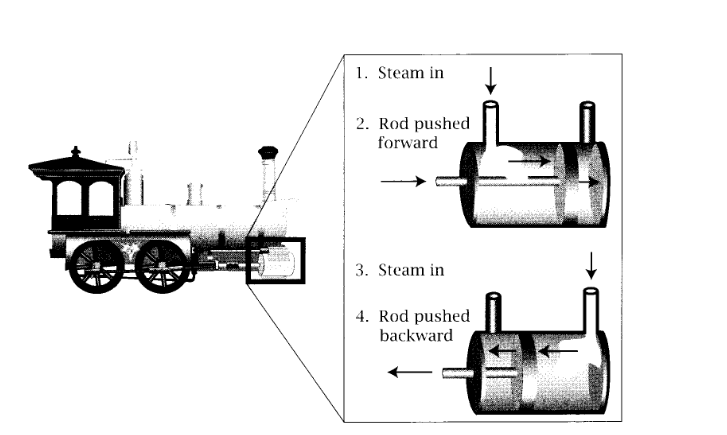
\includegraphics[scale=0.3]{trem.png}
  \end{center}
}



\frame{\frametitle{Não Conservação}
  \begin{itemize}
  \item O Calor não podia ser inteiramente reaproveitado.
  \item Experimento fracassado de ``Ericsson em 1853''.
  \end{itemize}
  \begin{center}
    \includegraphics[scale=0.2]{nytimes}
  \end{center}
}

\frame{\frametitle{Irradiação}
  \begin{itemize}
  \item Calor se propaga por irradiação.
  \end{itemize}
}

\frame{\frametitle{História do Calor}
  \begin{itemize}
  \item Trabalho podia ser transformado em Calor. Experimentos de
    Joule:
    \begin{itemize}
    \item Energia Potencial em Calor
    \item Energia Elétrica em Calor
    \end{itemize}
  \end{itemize}
  \begin{center}
    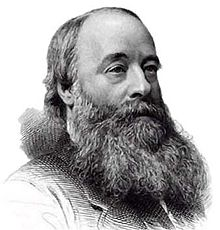
\includegraphics[scale=0.5]{joule}
  \end{center}

}


\frame{\frametitle{1$^{a}$ Lei da Termodinâmica} A energia interna de
  um sistema:

$$U=q+w$$

onde $q$ é o calor trocado e $w$ o trabalho realizado é conservada.

(Meyer 1842)

}


\frame{\frametitle{Teoria Cinética dos Gases}


  Os átomos possuem graus de liberdade que podem ser utilizados para
  armazenar energia.

  \begin{itemize}
  \item Matéria é composta por átomos.
  \item Calor é uma forma de energia trocada devido aos movimentos
    moleculares.
  \item A energia eletromagnética influencia os átomos e explica a
    troca de calor por irradiação.
  \end{itemize}
}

\frame{\frametitle{Teoria Cinética dos Gases} A teoria cinética
  consegue prever o comportamento de gases precisamente além de
  permitir interpretar a temperatura:

$$\frac{3}{2}kT=\frac{m\langle v^2 \rangle}{2}$$

$k$ constante de Boltzmann.  }


\frame{\frametitle{Teoria Quântica}

  A Teoria Quântica prevê que os níveis de energia que um sistema
  fechado pode possuir são discretos. Esta constatação tem importantes
  consequências para a Termodinâmica.

  O conhecimento apenas dos possíveis níveis de energia nos permite
  prever a maior parte das propriedades termodinâmicas.

$$U=\sum_i N_i \epsilon_i$$
}


\frame{\frametitle{Por que o Calor Flui?}


  Em primeiro lugar quanto maior for a energia de um sistema, maior o
  número de estados acessíveis.

  {\bf Def. } Considere um sistema com $N$ partículas e com 3 níveis
  possíveis de energia: $\epsilon=\epsilon_o, 2\epsilon_o,
  3\epsilon_o$. Suponha agora que temos 3 partículas e um valor de
  energia total de $3 \epsilon$. Quanto vale a multiplicidade $W$
  deste sistema? E para o caso $W=6\epsilon_o$?

}

\frame{\frametitle{Fluxo de Energia}

  A energia se distribui igualmente pois isto maximiza a
  multiplicidade. Considere dois subsistemas formados cada um por 3
  partículas e uma energia interna de $12\epsilon_o$. Calcule as
  multiplicidades para o caso em que a energia se distribui de forma
  simétrica e para o caso em que isto não ocorre. Se convença que a
  multiplicidade do primeiro caso é maior.  }

\frame{\frametitle{Fluxo de Energia} Considere dois sistemas que
  possuem apenas dois níveis de energia: $\epsilon_o$ e
  $\epsilon_1$, cada sistema possui 10 partículas. Considere a 
situação em que o sistema $A$ possui duas partículas no estado excitado
e $B$ 4 partículas.

$$W=\frac{ 10!}{8!2!} \frac{10!}{4!6!}=9450$$

Coloque os dois sistemas em contato o que vai maximizar a multiplicidade?

$$W=\frac{ 10!}{3!7!} \frac{10!}{3!7!}=14400$$

}


\frame{\frametitle{Fluxo de Energia} Considere dois sistemas que
  possuem apenas dois níveis de energia: $\epsilon_o$ e
  $\epsilon_1$. Considere a 
situação em que o sistema $A$ possui 10 partículas 
e duas partículas no estado excitado
e $B$ 4 partículas e duas partículas no estado excitado.

$$W=\frac{ 10!}{8!2!} \frac{4!}{2!2!}=270$$

Coloque os dois sistemas em contato o que vai maximizar a multiplicidade?

$$W=\frac{ 10!}{3!7!} \frac{4!}{3!1!}=480$$

}

\frame{\frametitle{Observações}
  \begin{itemize}
  \item O fluxo de energia maximiza a multiplicidade, mas nem sempre
    equaliza as energias.
  \item A temperatura é que acaba por ser igualada em quaisquer
    sistemas em contato. Sistemas em contato térmico tendem a possuir
    a mesma temperatura.
  \end{itemize}
}
\end{document}